\def\systemnameRaw{}
\def\systemname{\systemnameRaw\xspace}

\PassOptionsToPackage{table,xcdraw,dvipsnames}{xcolor}
\PassOptionsToPackage{hyphens}{url}
\PassOptionsToPackage{unicode}{hyperref}
\PassOptionsToPackage{naturalnames}{hyperref}

\documentclass[sigplan,screen]{acmart}
\settopmatter{printacmref=false, printccs=true, printfolios=false}


\copyrightyear{2021}
\acmYear{2021}
\setcopyright{acmcopyright}\acmConference[PaPoC'21]{8th Workshop on Principles and Practice of Consistency for Distributed Data}{April 26, 2021}{Online, United Kingdom}
\acmBooktitle{8th Workshop on Principles and Practice of Consistency for Distributed Data (PaPoC'21), April 26, 2021, Online, United Kingdom}
\acmPrice{15.00}
\acmDOI{10.1145/3447865.3457964}
\acmISBN{978-1-4503-8338-7/21/04}


















\renewcommand{\arraystretch}{1.25} %



\usepackage{hhline} %


\usepackage{color}
\usepackage{enumitem}
\usepackage{float}
\usepackage{graphicx}
\hypersetup{
    colorlinks=false,
    pdfborder={0 0 0},
}
\usepackage{listings}
\usepackage{multirow}
\usepackage{nicefrac}



\usepackage{sidecap}
\usepackage{subcaption}
\usepackage{verbatim}


\lstset{
    float=[*],
    language=C,                %
    basicstyle=\scriptsize\ttfamily,
    stringstyle=\color{sh_string},
    keywordstyle = \color{sh_keyword}\bfseries,
    commentstyle=\color{sh_comment}\itshape,
    numbers=left,                   %
    numberstyle=\scriptsize,        %
    stepnumber=1,                   %
    numbersep=5pt,                  %
    backgroundcolor=\color{white},  %
    showspaces=false,               %
    showstringspaces=false,         %
    showtabs=false,                 %
    xleftmargin=2em,                %
    frame=lines,         %
    framexleftmargin=1.5em,         %
    framexbottommargin=0em,         %
    morekeywords={in,not,and,or},
    prebreak=\space,                %
    postbreak=\mbox{{\color{blue}\scriptsize$\hookrightarrow$}}, %
    breaklines=true,                %
    breakatwhitespace=false,        %
    tabsize=2,                      %
    captionpos=t,                   %
    escapeinside={@}{@}             %
}
\lstdefinelanguage{javascript}{
  keywords={typeof, new, true, false, catch, function, return, null, catch, switch, var, if, in, while, do, else, case, break},
  keywordstyle=\color{blue}\bfseries,
  ndkeywords={class, export, boolean, throw, implements, import, this},
  ndkeywordstyle=\color{black}\bfseries,
  identifierstyle=\color{black},
  sensitive=false,
  comment=[l]{//},
  morecomment=[s]{/*}{*/},
  commentstyle=\color{purple}\ttfamily,
  stringstyle=\color{red}\ttfamily,
  morestring=[b]',
  morestring=[b]"
}





%%%%%%%%%%%%%%%%%%%%%%
% Comments
%%%%%%%%%%%%%%%%%%%%%%
\newif\ifshowcomment
\showcommenttrue
% \showcommentfalse

\ifshowcomment

\newcommand{\todo}[1]{\noindent\textsf{\color{NavyBlue}{[{{\bf \scalebox{0.75}{\fbox{ToDo}}}: {\it#1}]}}}}
\newcommand{\newtext}[1]{\textcolor{blue}{#1}} % Added new texts
\newcommand{\modtext}[1]{\textcolor{red}{#1}}  % Modified texts
\newcommand{\boris}[1]{\noindent\textsf{\color{Violet}{[{{\bf \scalebox{0.75}{\fbox{Boris}}}: {\it#1}]}}}}
\newcommand{\vijay}[1]{\noindent\textsf{\color{purple}{[{{\bf \scalebox{0.75}{\fbox{Vijay}}}: {\it#1}]}}}}
\newcommand{\vasilis}[1]{\noindent\textsf{\color{orange}{[{{\bf \scalebox{0.75}{\fbox{Vasilis}}}: {\it#1}]}}}}
\newcommand{\arpit}[1]{\noindent\textsf{\color{magenta}{[{{\bf \scalebox{0.75}{\fbox{Arpit}}}: {\it#1}]}}}}
\newcommand{\antonis}[1]{\noindent\textsf{\color{OliveGreen}{[{{\bf \scalebox{0.75}{\fbox{Antonis}}}: {\it#1}]}}}}

\else
\newcommand{\newtext}[1]{#1} 
\newcommand{\modtext}[1]{#1}
\newcommand{\todo}[1]{}
\newcommand{\antonis}[1]{}
\newcommand{\boris}[1]{}
\newcommand{\vijay}[1]{}
\newcommand{\arpit}[1]{}
\newcommand{\vasilis}[1]{}
\fi

\newcommand{\y}[1]{#1}
% \newcommand{\y}[1]{{\color{blue} #1}\normalcolor}
% \newcommand{\y}[1]{{#1}}

%%%%%%%%%%%%%%%%%%%%%%%%%%%%%%%%%%%%%%
%%% CUSTOM COMMANDS
%%%%%%%%%%%%%%%%%%%%%%%%%%%%%%%%%%%%%%


%%%%%%%%%%%%%%%%%%%%%%
% Emphasized space-efficient bullets start
%%%%%%%%%%%%%%%%%%%%%%
\newcommand{\beginitem}[1]{\noindent $\succ$ \textit{#1}}



%%%%%%%%%%%%%%%%%%%%%%
% Floor and ceiling commands
%%%%%%%%%%%%%%%%%%%%%%
\newcommand{\floor}[1]{\lfloor #1 \rfloor}
\newcommand{\ceil}[1]{\lceil #1 \rceil}

%%%%%%%%%%%%%%%%%%%%%%
% Make full capitalized words less intrusive
%%%%%%%%%%%%%%%%%%%%%%
\newcommand{\CAP}[1]{\scalebox{0.85}{#1}}

%%%%%%%%%%%%%%%%%%%%%%
% circled character
%%%%%%%%%%%%%%%%%%%%%%
\newcommand*\circled[1]{\tikz[baseline=(char.base)]{
            \node[shape=circle,draw,inner sep=0.5pt] (char) {#1};}}


%%%%%%%%%%%%%%%%%%%%%%%%%
%% Squish lists
%% Usage: 
%%   \squishlist
%%     \item ..
%%   \squishend
%%%%%%%%%%%%%%%%%%%%%%%%%
\newcommand{\squishlist}{
 \begin{list}{$\bullet$}
  { \setlength{\itemsep}{2pt}
     \setlength{\parsep}{0pt}
     \setlength{\topsep}{2pt}
     \setlength{\partopsep}{0pt}
     \setlength{\leftmargin}{1em}
     \setlength{\labelwidth}{1em}
     \setlength{\labelsep}{0.5em} } 
}

\newcommand{\squishlistContrib}{ %
 \begin{list}{$\bullet$}
  { \setlength{\itemsep}{2pt}
     \setlength{\parsep}{0pt}
     \setlength{\topsep}{2pt}
     \setlength{\partopsep}{0pt}
     \setlength{\leftmargin}{1em}
     \setlength{\labelwidth}{1em}
     \setlength{\labelsep}{0.5em} }
}
\newcommand{\squishend}{ \end{list}  }


\newcommand{\squishenum}{\begin{enumerate}[itemsep=0.5pt,parsep=0pt,topsep=0pt,partopsep=0pt,leftmargin=1.5em,labelwidth=1em,labelsep=0.5em]{}}
\newcommand{\squishenumend}{\end{enumerate}}


%%% URLs
\newcommand\myurl[2]{\url{#1}}

\renewcommand{\floatpagefraction}{0.95}

\newcommand{\captionfonts}{\small}
\makeatletter  % Allow the use of @ in command names
\long\def\@makecaption#1#2{%
  \vskip 0.1in
  \sbox\@tempboxa{{\captionfonts #1: #2}}%
  \ifdim \wd\@tempboxa >\hsize
    {\captionfonts #1: #2\par}
  \else
    \hbox to\hsize{\hfil\box\@tempboxa\hfil}%
  \fi
  \vskip 0in}
\makeatother   % Cancel the effect of \makeatletter

% Theorems
\newtheorem{mydefinition}{Definition}
\newtheorem{mytheorem}{Theorem}
\newtheorem{definition}{Definition}
\newtheorem{theorem}{Theorem}

%%% Alignment
%\begin{center/flushright/flushleft}
%...
%\end{center/flushright/flushleft}


%% Margins
%  \usepackage[margin=0.5in]{geometry}

%%% Paragraphs and other breaks
% Paragraphs are separated by a blank line.
% You can force a new line using \\
% To force a new page, use \newpage or \clearpage

%%%% Other spacing
% Force a space using ∼
% Add space using \hspace{1in} or \vspace{1in}
% Fill space using \hfill or \vfill

\def\colorhl{\cellcolor[HTML]{C0C0C0}}
\def\hlrow{\rowcolor[HTML]{C0C0C0}}
\def\colorgrey{\cellcolor[HTML]{e6e6e6}}
\def\greyrow{\rowcolor[HTML]{e6e6e6}}
\def\custvspace{\vspace{0.4em}}
\newcommand{\qt}[1]{``#1''}
\def\colorhl{\cellcolor[HTML]{C0C0C0}} % highlight a the top cells of a table

%%%%%%%%%%%%%%%%%%%%%%
% Instead of using sub-subsections 
% use the following as an emphasized 
% first sentence of a new paragraph
%%%%%%%%%%%%%%%%%%%%%%
\newcommand{\beginbsec}[1]{\custvspace\noindent\textbf{#1.}}

\def\custevalvspace{\vspace{0.3em}}
\newcommand{\beginbseceval}[1]{\custevalvspace\noindent\textbf{$\succ$ #1.}}

\def\RDMA{RDMA}
\def\RMW{RMW}
\def\RMWs{RMWs}
\def\odlib{\emph{Odys\-sey}}
\def\pnum{ten}

\def\LTO{LTO}
\def\LPKO{LPKO}
\def\DTO{DTO}
\def\DPKO{DPKO}
\newcommand{\figref}[1]{Figure~\ref{#1}}
\newcommand{\secref}[1]{Section~\ref{#1}}
\newcommand{\tabref}[1]{Table~\ref{#1}}
%%%%%%%%%%%%%%%%%%%%
%%%% Latin Abbreviations 
%%%%%%%%%%%%%%%%%%%%
\def\etal{et~al.} % ``and others'', ``and co-workers''
\def\eg{e.g.,~} % ``for example''
\def\ie{i.e.,~} % ``that is'', ``in other words''
\def\etc{etc} % ``and other things'', ``and so forth''
\def\cf{cf.~} % ``compare''
\def\viz{viz.~} % ``namely", ``precisely''
\def\vs{vs.~} % ``against"

% \newcommand\eg[]{e.g., }
% \newcommand\ie[]{i.e., }
% \newcommand\eg[0]{e.g.\ }
% \newcommand\ie[0]{i.e.\ }
% \newcommand\et[0]{et al.\ }

%%%%%%%%%%%%%%%%%%%%
%%%% Spell check
%%%%%%%%%%%%%%%%%%%%

% if you want to spell-check your document, you can use the command-line aspell, hunspell (preferably), or ispell programs.
% E.g.:
%       ispell yourfile.tex
%   aspell --mode=tex -c yourfile.tex
%   hunspell -l -t -i utf-8 yourfile.tex

%% Word cound
%If you want to count words you can, again, use LyX or convert your LaTeX source to plain text and use, for example, UNIX wc command:
% detex yourfile | wc

%%%%%%%%%%%%%%%%%%%%
%% Hyphenated words
%%%%%%%%%%%%%%%%%%%%
%\hyphenation { hy-phen-a-tion mar-vel-ous-ly }


\def\ourtitle{Towards the Synthesis of Coherence/Replication Protocols from Consistency Models via Real-Time Orderings}
\title[Synthesis of Coherence/Replication Protocols from Consistency Models] { \ourtitle}
\author{}
\date{}



\begin{document}
\author{Vasilis Gavrielatos, Antonios Katsarakis, Vijay Nagarajan}
\affiliation{%
  \institution{The University of Edinburgh\\
  FirstName.LastName@ed.ac.uk}
}




%%
%% The code below is generated by the tool at http://dl.acm.org/ccs.cfm.
%% Please copy and paste the code instead of the example below.
%
\begin{CCSXML}
<ccs2012>
<concept>
<concept_id>10010520.10010521.10010537.10003100</concept_id>
<concept_desc>Computer systems organization~Cloud computing</concept_desc>
<concept_significance>300</concept_significance>
</concept>
<concept>
<concept_id>10010520.10010575.10010577</concept_id>
<concept_desc>Computer systems organization~Reliability</concept_desc>
<concept_significance>300</concept_significance>
</concept>
<concept>
<concept_id>10010520.10010575.10010578</concept_id>
<concept_desc>Computer systems organization~Availability</concept_desc>
<concept_significance>300</concept_significance>
</concept>
<concept>
<concept_id>10011007.10010940.10010992.10010993.10010996</concept_id>
<concept_desc>Software and its engineering~Consistency</concept_desc>
<concept_significance>300</concept_significance>
</concept>
</ccs2012>
\end{CCSXML}

\ccsdesc[300]{Computer systems organization~Cloud computing}
\ccsdesc[300]{Computer systems organization~Reliability}
\ccsdesc[300]{Computer systems organization~Availability}
\ccsdesc[300]{Software and its engineering~Consistency}

%
% Keywords. The author(s) should pick words that accurately describe
% the work being presented. Separate the keywords with commas.
\keywords{Fault-tolerant; Replication; Consistency; Availability; Throughput; Latency; Linearizability; RDMA}

\begin{abstract}
% \subsection*{Abstract}
Get/Put Key-Value Stores (KVSes) rely on replication protocols to enforce consistency and guarantee availability.
Today's modern hardware, with manycore servers and RDMA-capable networks, challenges the conventional wisdom on protocol design.
In this paper, we investigate the impact of modern hardware on the performance of strongly-consistent replication protocols.

First, we create an informal taxonomy of replication protocols, based on which we carefully select 10 protocols for analysis.
Secondly, we present Odyssey, a framework tailored towards protocol implementation for multi-threaded, RDMA-enabled, in-memory, replicated KVSes. We implement all 10 protocols over Odyssey, and perform the first apples-to-apples comparison of replication protocols over modern hardware.

Our comparison characterizes the protocol design space, revealing the performance capabilities of different classes of protocols on modern hardware. 
Among other things, our results 
demonstrate that some of the protocols that were efficient in yesterday's hardware are not so today because they cannot take advantage of the abundant parallelism and fast networking present in modern hardware. Conversely, some protocols that were inefficient in yesterday's hardware are very attractive today.
We distill our findings in a concise set of general guidelines and recommendations for protocol selection and design in the era of modern hardware.
% While protocols that can scale on modern hardware can 
% that are present in modern hardware.
\end{abstract}

% The characterization demonstrates that to achieve high throughput and low latency, protocols must take advantage of the abundant parallelism and the fast networking that are present in modern hardware.
% Exemplifying this paradigm shift is the drastic impact of multi-threading on the relative performance of protocols.
% We distill our findings in a concise set of general guidelines and recommendations for protocol selection and protocol design in the era of modern hardware.

% mustprotocol design in the era of modern hardware must take into  account the abundant parallelism and the fast networking
% The impact of modern hardware on protocol performance is exemplified
% in the era of modern hardware.
% Furthermore, we demonstrate that modern hardware challenges the conventional wisdom in protocol design, shifting the focus towards parallelism. Exemplifying this paradigm shift is the drastic impact of multi-threading on the relative performance of protocols. 
% For instance, ZAB outperforms Classic Paxos by more than 2x when both are single-threaded, but the result is inverted when they are multi-threaded.

% The insights gained from viewing protocols through a hardware-aware lens, inform both protocol selection and protocol design

% Our comparison characterizes the protocol design space, revealing the performance capabilities of different classes of protocols and the relative importance of design decisions in the era of modern hardware. The insights gained from viewing protocols through a hardware-aware lens, inform both protocol selection and protocol design

% No-SQL Key-Value Stores (KVSes), that underpin modern online services, rely on strongly-consistent protocols to offer a highly available read / (conditional) write interface.
% The ubiquitous 
% Get/Put Key-Value Stores (KVSes) rely on replication protocols to enforce consistency and guarantee availability.
% % Over the last 30 year, numerous such protocols have been proposed attempting to maximize performance. 
% Today's modern hardware, with manycore servers and RDMA-capable networks, challenge the conventional wisdom on protocol design.
% %radically change the requirements of protocol design.
% % Plainly, a protocol that was efficient 10 years ago for a four-core server may not be so today, if it cannot scale across cores. Vice versa, a once slow protocol may be very efficient today, if it is scalable.
% % Today's modern hardware, with manycore servers with tens of cores and RDMA-capable networks challenge the traditional wisdom on protocol design.
% % In this paper, we pose two questions. How do existing protocols perform on modern hardware and what are the best design practices? 
% In this paper we investigate the impact of modern hardware on the performance of existing protocols and on design practices.

% First we create an informal taxonomy of replication protocols, based on which we carefully select 10 protocols for analysis.
% % : ZAB, Multi-Paxos, 
% % Derecho, CHT, CHT-multi-ldr, CRAQ, Classic Paxos, All-aboard Paxos, ABD and Hermes.
% Secondly, we present Pixie, a framework tailored towards protocol implementation for multi-threaded, RDMA-enabled, in-memory, replicated KVSes. We implement all 10 protocols over Pixie, and perform the first apples-to-apples comparison of replication protocols over modern hardware.

% The results of the comparison demonstrate that modern hardware forces us to shift the focus to parallelism and load balance instead of message rounds per request. Exemplifying this paradigm shift is the impact of multi-threading on the relative performance of protocols. 
% For instance, ZAB outperforms Classic Paxos (CP) by more than 2x when both are single-threaded, but the result is inverted when they are multi-threaded.






%\end{abstract}

% A category with the (minimum) three required fields
%\category{D.4.1}{Operating Systems}{Process Management}, {Multiprocessing}
%\category{D.4.4}{Operating Systems}{Communications Management}, {Network Communication}
%\category{D.4.7}{Operating Systems}{Organization and Design}, {Distributed Systems}
%\terms{Theory}
%\keywords{Design, Reliability, Performance, Security, Web, } % NOT required for Proceedings

\maketitle




\section{Introduction}

This work focuses on \qt{shared memory} systems that provide a read/write interface to the programmer. Such systems are ubiquitous in both computer architecture and  distributed systems. Prominent examples include shared memory multiprocessors (SMPs), GPUs, NoSQL Databases~\cite{twitter:2016}, coordination services\cite{Hunt:2010}, and software-based DSMs~\cite{Keleher:1994}.

Such systems commonly replicate data -- sometimes for performance (through caching), sometimes for fault tolerance and sometimes for both.
To enable reasoning in the presence of replication, a \emph{memory consistency model} (\emph{\mcm}) is specified as part of the system's interface, providing the rules that dictate what values a read can return.
In order to enforce the \mcm, the system deploys a protocol which ensures that the replicas behave in accordance to the \mcm. This protocol is called \emph{coherence protocol} in computer architecture and \emph{replication protocol} in distributed systems. We simply refer to it as \emph{the protocol}.

The \mcm\ specifies the behaviour of the system when executing parallel programs by enumerating all patterns through which parallel programs can synchronize.
For example, an \mcm\  $CM_a$ can guarantee the synchronization pattern of \figref{fig:intro-ex}a (commonly known as \qt{producer-consumer}). Specifically, in \figref{fig:intro-ex}a, process P1 writes object $x$ and then $y$, while process P2 reads $y$ and then $x$. 
$CM_a$ guarantees that if P2's read to $y$ returns the write of P1, then P2's read to $x$ will also return the write of P1 (\ie $x=1$).


\begin{figure}[t]
  \centering
  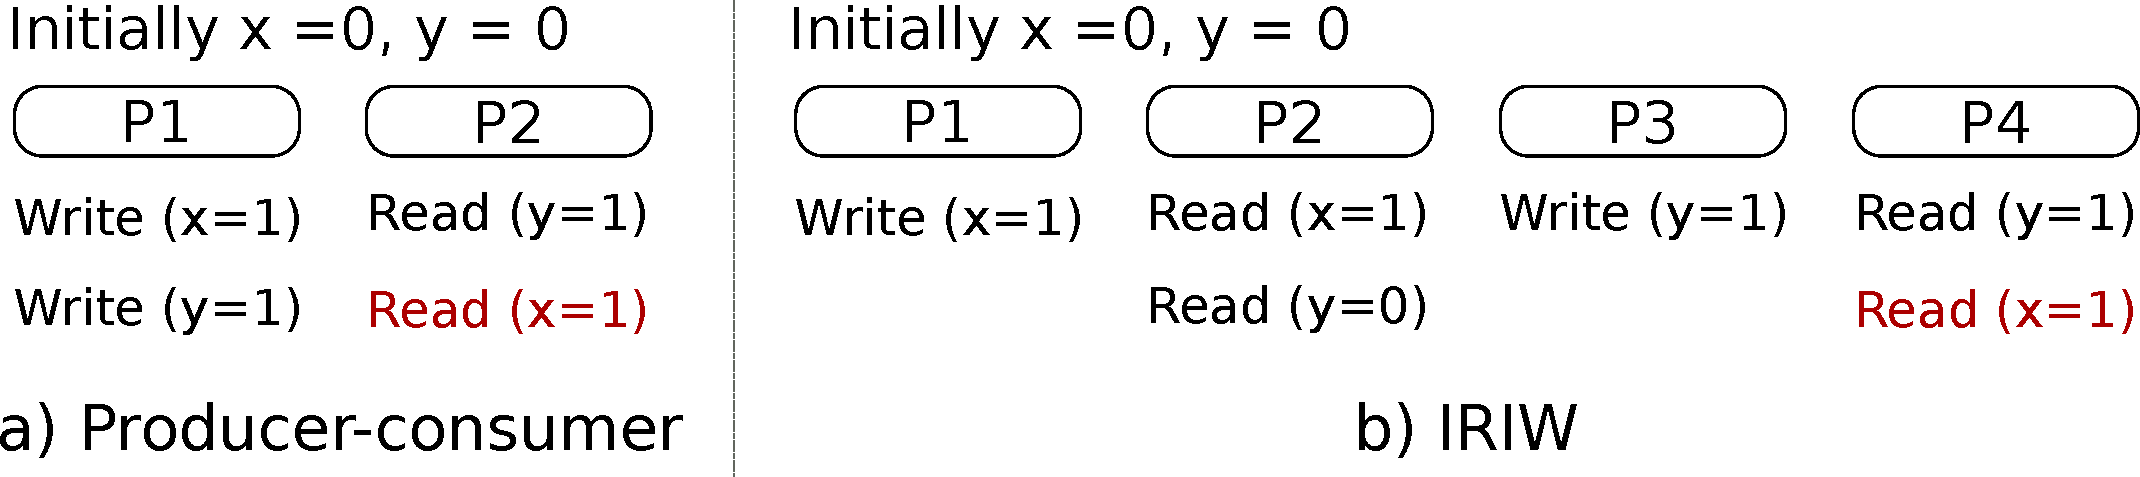
\includegraphics[width=0.48\textwidth]{1_figures/intro-example.pdf}
  \caption{a) The producer-consumer synchronization pattern mandates that if P2 reads P1's write to $y$, then it must also read P1's write to $x$. b) The independent-reads independent-writes (IRIW) pattern mandates that if P2 sees P1's writes but not P3's and P4 sees P3's write, then P4 must see P1's write. }
  \label{fig:intro-ex}
\end{figure}
\custvspace
The \mcm\ is thus  a contract between the programmers and the designers. While programmers must understand the behaviour of the system, the designers must understand how to implement that behaviour.
Problematically, enforcing the \mcm\ is very challenging. 
For instance, consider two well known \mcms: TSO~\cite{Owens:2009} and Causal Consistency (CC)~\cite{Petersen:1997}. TSO enforces both \figref{fig:intro-ex}a and b while CC enforces \figref{fig:intro-ex}a but not b.
Given this information, how is the designer to implement a correct and efficient protocol for either \mcm?
Crucially, how is the designer to differentiate between the two models? E.g., how can one exploit that \figref{fig:intro-ex}b need not be enforced in the CC protocol? 

\y{
Our overarching vision is to automate the above task: given a target \mcm\ we envision a software tool that can produce an efficient protocol. 
We argue that to create this tool we need one additional level of abstraction which can act as an intermediary between the \mcm\ and the protocol.
That is: (1) we must be able to automatically translate any \mcm\ to this abstraction; and (2) we must also be able to map the abstraction itself 
into protocol design choices.
In this work, we take a step towards actualizing our vision, by  proposing such an abstraction and, most crucially, presenting the mapping from \mcms\ to this abstraction. 
We also informally relate the abstraction to protocol design choices. 

}

To create this abstraction, we observe that a shared memory system, be it a multiprocessor or a geo-replicated Key-Value Store (KVS), can be abstracted through the model of \figref{fig:intro-mod}, which depicts a set of processes executing a parallel program. 
Each process inserts its memory operations to a structure we call the \emph{reorder buffer (\rob)},  allocating one \rob\ entry per operation.
The \emph{memory system} executes the operations it finds in the \rob\ and writes back the response of each operation in-place in its dedicated entry.

A process models a client of a KVS or a core of a multiprocessor. The \rob\ abstracts the core's load-store queue or a software queue that a KVS must maintain to keep track of incoming requests.
The memory system is modelled as a distributed system comprising a set of \emph{nodes}, where each node contains a controller and a memory.
The nodes model the private caches of the multiprocessor or the geo-replicated memory servers of the KVS. Finally the network of the memory system can be thought of as the Network-on-Chip or as the WAN.

We observe that protocols of real systems enforce various consistency models using two widgets: 1) the \rob\ that allows for the reordering of operations; and 2) the memory system which determines how a read or a write executes, \ie how it propagates to each of the replicas. 
We propose two sets of mathematical rules to abstract protocols, one that can abstract the reorderings of the \rob\ and one that can abstract the propagation rules of the memory system.

\begin{figure}[t]
  \centering
  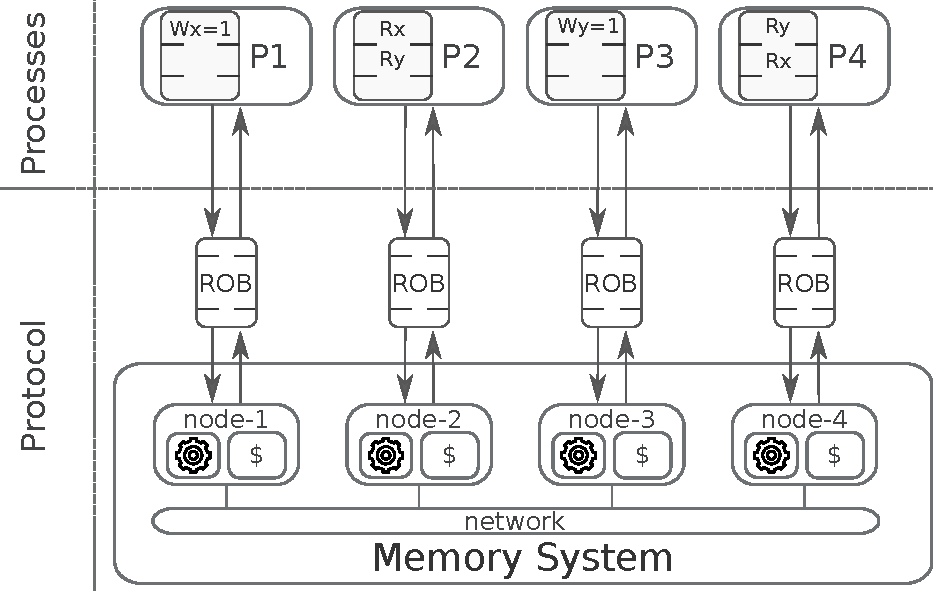
\includegraphics[width=0.45\textwidth]{1_figures/intro-model.pdf}
  \caption{The model of a shared memory system. Processes P1-P4 execute the IRIW pattern of \figref{fig:intro-ex}b. }
  \vspace{-1em}
  \label{fig:intro-mod}
\end{figure}

Specifically, we model the \rob\ using four rules named \emph{program-order real-time orderings} (\emph{\prts}).
The $\prtwr$ \prt\ mandates that when write $w$ precedes read $r$ in a program execution, then $r$ can begin executing in the memory system only after $w$ has completed.
Similarly, we define $\prtww,\prtrr, \prtrw$, for the rest of the combinations between reads and writes.
To summarize, we model an \rob\ by specifying the subset of the four \prts\ it enforces. 

We model the memory system using four rules named \emph{synchronization real-time orderings} (\emph{\srts}).
The $\rtwr$ \srt\ mandates that if write $w$ to object $x$ completes before read $r$ to object $x$ in real time, then $r$ must observe $w$.
Similarly, we define $\rtww, \rtrr, \rtrw$.
To summarize we model a memory system by specifying the subset of the four \srts\ it enforces.

We refer to \prts\ and \srts\ as \emph{real-time orderings} (\emph{\rts}).
The eight \rts\ comprise our designer-centric intermediate abstraction of the protocol. 

\y{
While the \rts\ have been employed by other works in the past to model consistency models or protocols (\S\ref{sec:related}), this work is the first to present a 
mapping from \mcms\ to the \rts. That is, given any \mcm, we provide the set of minimal \rts\ that enforce it. 
Crucially, this mapping, along with relating the \rts\ with protocol implementation techniques, pave the way for automating protocol design.
}

Using this mapping from \mcms\ to \rts, we now revisit the questions we posed on \figref{fig:intro-ex}. Specifically, \prts\ $\prtww$ and $\prtrr$ and the \srt\ $\rtwr$ suffice to enforce the producer-consumer pattern (discussed in \secref{sec:rt-cons:reg-ex}). 
Informally, $\prtww$ mandates that writes from the same process must be executed in the order intended by the program; $\prtrr$ mandates the same for reads; $\rtwr$ mandates that a read must be able to return the value of the latest completed write (from any process).
To also enforce the IRIW pattern, $\rtrr$ is required (discussed in \secref{sec:rt-cons:irreg}). Informally, $\rtrr$ mandates that if a read returns the value of write $w$, then any later read must also be able to return the value of write $w$.

\beginbsec{Contributions}
In summary, in this work we make the following contributions:
\squishlistContrib
\item 
We propose and formalize eight \rts\ for mathematically modelling consistency enforcement protocols, serving as an intermediate abstraction between the \mcm\ and the protocol implementation (\S\ref{sec:rt}).
\item
We create a mapping from \mcms\ to \rts, specifying the minimal set of \rts\ sufficient to enforce any \mcm\ (\S\ref{sec:rt-cons}) \y{and vice versa, specifying the \mcm\ enforced by any set of \rts\ (\S\ref{sec:rt-to-cons})}. 
\item
We informally map \rts\ to protocol implementation techniques (\S\ref{sec:prot}).
\squishend

























\section{Preliminaries}


In this section, we first establish the system model, then we describe the notation we will use throughout the paper and finally we discuss how executions are modeled. %

\subsection{System Model} \label{sec:sysmod}
\figref{fig:intro-mod} illustrates our system model.
Specifically, there is a set of $P$ \emph{processes}, each of which executes a program and there is a \emph{protocol} which enforces the \mcm. %
The \emph{protocol} is comprised of a set of \emph{reorder buffers} (\robs) and the \emph{memory system}.
The \emph{memory system} stores a set $X$ of shared \emph{objects}, each of a unique name and value.
A memory operation (or simply \emph{operation}) can be either a read or a write of an object. A read returns a value and a write overwrites the value of the object and returns an ack.

\beginbsec{\robs}
 The \robs\ are used to facilitate communication between the processes  and the protocol. %
There are three events in the lifetime of an operation within the \rob: \emph{issuing},  \emph{begin} and \emph{completion}. Specifically, 
we write that a process \qt{issues an operation}, when the operation is first inserted in the \rob. A process pushes operations in the \rob\ in the order that they are encountered within its program. 
We refer to this order as the \emph{program order}.
Furthermore, we write that \qt{an operation begins} when the memory system begins executing the operation. In this case the memory system marks the operation's \rob\ entry as \emph{beginned}. 
Similarly, we write that \qt{an operation completes} when the memory system has finished executing the operation. In this case, the memory system marks the operation's \rob\ entry as \emph{completed} (and writes back the result if it is a read).

Notably, a process can use the value returned by a read, as soon as the read is marked \emph{completed} by the memory system, irrespective of whether preceding operations are completed.
An operation is removed from the \rob, if all three conditions hold: 1) it is the oldest operation, 2) it is completed and 3) the process has consumed its value, if it is a read.

\beginbsec{Memory system}
We model the memory system as a distributed system comprised of a set of \emph{nodes}, where each node contains a controller and a memory.
Furthermore, each node is connected to one \rob, from which it reads the operations that must be executed. The controller of each node is responsible for the execution of the operations. The memory of each node stores every object in $X$.

















\subsection{Notation}
The notation used throughout this paper is the one used by Alglave \etal~\cite{Alglave:2014}. We repeat it here 
for completeness.
The notation is based on relations.
Specifically, we will denote the transitive closure of $r$ with $r^\ast$ and the composition of $r1$, $r2$ with $r1;r2$. 
We say that $r$ is \emph{acyclic} if its transitive closure is irreflexive and we denote by writing \emph{acyclic(r)}.
Finally, we say that $r$ is a \emph{partial order}, when $r$ is transitive and irreflexive. We say that a partial order $r$ is a \emph{total order} over a set $S$, if for every $x,y$ in $S$, it is that $(x, y) \in r \orm (y,x) \in r$.

We use small letters to refer to memory operations (\eg $a$, $b$, $c$ \etc).
In figures that show executions (\eg \figref{fig:synpat}), we denote a write with $Wx = val$ where $x$ is the object to be written and $val$ is the new value.
Similarly, reads are represented as $Rx = val$, where $val$ is the  value returned.
When required relations between operations are denoted with red arrows in figures.


\subsection{Modelling executions}
To model executions, we use the framework created by Alglave \etal~\cite{Alglave:2014}, introducing minor changes where necessary. 
Specifically, we model an execution as a $tuple(M$, $po$, $rf$, $hb$, $RL)$.
M is the set of memory operations included in the execution, $po, rf$ and $hb$ are relations over the operations and $RL$ is a set of relations $rl$ over the operations.



\beginbsec{Execution relations ($\mathbf{po, rf, hb}$ and $\mathbf{rl}$)}
The \emph{program order} $po$ relation is a total order over the operations issued by a single process, specifying the order in which memory operations are ordered in the program executed by the process. Operations are issued by a process in this order. Only operations from the same process are ordered. For two operations $a, b$ from process $i \in P$,  if $a$ is issued before $b$ then $(a, b) \in po$. 


\custvspace\noindent
The \emph{reads-from} $rf$ relation contains a pair for each read operation in $M$, relating it with a write on the same object.
For the pair $(a, b) \in rf$, it must be that $a$ is a read that returns the value created by the write $b$, \ie $a$ \emph{reads-from} $b$.

\custvspace\noindent
The \emph{happens-before} $hb$ relation is a partial order over all operations, specifying the real-time relation of operations.
Specifically, for two operations $a, b$, if $(a, b) \in hb$, then that means that $a$ completes before $b$ begins. %

\custvspace\noindent
Finally, the \emph{read-legal} $rl$ relation is a total order over all operations, with the restriction that $acyclic(rl \cup rf)$.
Given the $rf$ of an execution $E$, it is often possible to construct more than one $rl$. We associate each execution $E$, with a set $RL$ which contains every $rl$ that can be constructed from $E$. 
For each $rl \in RL$, we derive the following relations.

\beginbsec{Relations derived from $\mathbf{rl}$ ($\mathbf{ws, fr, syn}$)}
The \emph{write-se\-riali\-za\-tion} $ws$ relation is a total order of writes to the same object that can be derived from $rl$, such that $ws \subseteq rl$. Intuitively, $ws$ captures the order in which writes to the same object serialize.

\custvspace\noindent
The \emph{from-reads} $fr$ relation connects a read to writes from the same object that precede the read in $rl$. Specifically, for every read $a$ and a write $b$ to the same object where $(a, b) \in rl$, then  $(a, b) \in fr$.
It follows that $fr$ is transitive and $fr \subseteq rl$. 

\custvspace\noindent
Finally, the \emph{synchronization} $syn$ relation combines the $rf, fr$ and $ws$ relations. Specifically, $syn$ is a partial order over operations on the same object defined as the transitive closure of the union of $rf, ws$ and $fr$, \ie $syn \triangleq (rf \cup ws \cup fr)^\ast$. 
Two operations on the same object are said to synchronize if one of them is a write. Formally, for any pair of operations $(a, b)$ on the same object, if at least one of $a, b$ is a write then it must be that $(a, b) \in syn \orm (b,a) \in syn$. If both $a, b$ are reads, then $(a, b) \in syn$ iff there exists a write $c$, such that $(a,c) \in syn \andm (c, b) \in syn$.


\beginbsec{Helper relations ($\mathbf{\potype, \syntype, \hbtype}$)}
Given the set of operations M, we define four relations $WW, WR, RR, RW$ over $M$ that contain all  write-write, write-read, read-read and read-write pairs found in $M$, respectively.
\tabref{tab:posyn} uses these four relations to define the $\potype$, $\syntype$ and $\hbtype$ relations. Specifically,
by taking the intersection of $po$ with each of $WW, WR, RR, RW$, we define $\poww, \powr,\porr, \porw$. We write $\potype$ as a placeholder that can be replaced by any of these four relations. Notably, every pair in $po$ is also in one of the $\potype$ relations. I.e.,
\begin{equation*}
    po \triangleq \poww \cup \powr \cup\porr \cup \porw
\end{equation*}

Similarly, we define $\synwr$ and $\synrr$. Note that we do not need to define $\synww$ and $\synrw$, because they would be the same as $ws$ and $fr$, respectively.
We write $\syntype$ as a placeholder for $ws, \synwr, \synrr, fr$.
We note that every pair in $syn$ is also in one of the $\syntype$ relations and that $rf$ is a subset of $\synwr$.
\begin{gather*}
    syn \triangleq ws \cup \synwr \cup \synrr \cup fr\\
    rf \subseteq \synwr
\end{gather*}
Finally, in the same spirit, we define the $\hbtype$ relations: $\hbww, \hbww, \hbrr,\hbrw$.








\section{Real-time orderings}\label{sec:rt}
In this section we introduce and formally define the \emph{real-time orderings} (\rts), through which we model the protocol.
There are two types of \rts: the program-order real-time orderings (\emph{\prts}) through which we model the operation of the \rob\ and the synchronization real-time orderings (\emph{\srts}), through which we model the operation of the memory system.
\tabref{tab:rt-mean} provides the definition of each of the eight \rts. 
Below we first describe the \prts\ and then the \srts.


\subsection{Program-order Real-time Orderings}


An execution \Exec\ is said to enforce the $\prtwr$ if:
\begin{equation*}
  \forall w,r \in M\ s.t.\ (w,r) \in \powr \rightarrow  (w,r) \in \hbwr
\end{equation*}%
Plainly, a read $r$ cannot begin before all writes that precede it in program order have completed. 
\tabref{tab:rt-mean} extends this definition to write-write, read-read and read-write pairs. When all four \prts\ are enforced then it follows that 
$po \subseteq hb$.




\begin{table}[t]
\centering
\resizebox{0.48\textwidth}{!}{
\begin{tabular}{|c|c|||c|c|}
\hline
\multicolumn{2}{|c|||}{\colorhl\textbf{\prts}}  & 
\multicolumn{2}{|c|}{\colorhl\textbf{\srts}}               \\ 
\hline
\hline
$\prtww$ & 
$\poww \subseteq \hbww$ 
&
$\rtww$ & 
$acyclic(\hbww \cup syn)$
\\ \hline

$\prtwr$ & 
$\powr \subseteq \hbwr$ 
&
$\rtwr$ & 
$acyclic(\hbwr \cup syn)$
\\ \hline

$\prtrr$ & 
$\porr \subseteq \hbrr$ 
&
$\rtrr$ & 
$acyclic(\hbrr \cup syn)$
\\ \hline

$\prtrw$ & 
$\porw \subseteq \hbrw$ 
&
$\rtrw$ & 
$acyclic(\hbrw \cup syn)$
\\ \hline 

\end{tabular}
}
\caption{The condition required to enforce each rt-ordering. }
\label{tab:rt-mean}
\end{table}






\subsection{Synchronization Real-time Orderings}
The synchronization real-time orderings (\srts) are constraints over operations to the same object.
There are four \srts: $\rtww, \rtwr, \rtrr, \rtwr$.
An execution \Exec\ enforces the \srt\ $\rtwr$ if there exists $rl \in RL$ such that:
\begin{equation*}
    acyclic(\hbwr \cup syn)
\end{equation*}
In other words the $\rtwr$ mandates that for a write $a$ and a read $b$ if $(a , b) \in \hbwr$, then it must be that $(b, a) \notin syn$.
\tabref{tab:rt-mean} describes the condition required to enforce each of the \srts.
A memory system is said to enforce an \srt, if that \srt\ is enforced in every execution that can be generated by the memory system.
Notably, a combination of the \srts\ can be enforced, for example $\rtww, \rtwr$ are both enforced when $acyclic (syn \cup \hbww \cup \hbwr)$. 
When all four \srts\ are enforced then linearizability is enforced~\cite{Herlihy:1990} (we expand on this on \secref{disc:lin}).












\section{Memory consistency models (\mcms)}\label{sec:cons}
In order to create a mapping from memory consistency models (\mcms) to the \rts\ we need to establish a formalism for the \mcms. In this section, we use the formalism of Alglave \etal\cite{Alglave:2014} to describe \emph{synchronization patterns} (\synpats) and assert that any \mcm\ $CM$ is defined as a set of \synpats\ $S_{CM}$. An execution enforces $CM$ iff it enforces every \synpat\ in $S_{CM}$.
Below we define what a \synpat\ is and what its enforcement entails. 






\begin{table}[t]
\centering
\resizebox{0.48\textwidth}{!}{
\begin{tabular}{|c|||c|||c|}
\hline
\colorhl\textbf{po-type}  & 
\colorhl\textbf{syn-type}&
\colorhl\textbf{hb -type}  
\\ 
\hline
\hline
$\poww$ $\triangleq$
$po \cap WW$ 
&
$ws$  $\triangleq$ 
$syn \cap WW$
&
$\hbww$ $\triangleq$ 
$hb \cap WW$ 
\\ \hline 

$\powr$ $\triangleq$ 
$po \cap WR$ 
&
$syn_{wr}$ $\triangleq$
$syn \cap WR$
&
$\hbwr$ $\triangleq$ 
$hb \cap WR$\\
\hline 

$\porr$ $\triangleq$ 
$po \cap RR$ 
&
$syn_{rr}$ $\triangleq$
$syn \cap RR$
&
$\hbrr$ $\triangleq$ 
$hb \cap RR$\\ \hline 

$\porw$ $\triangleq$ 
$po \cap RW$ 
&
$fr$ $\triangleq$ 
$syn \cap RW$
&
$\hbrw$ $\triangleq$ 
$hb \cap RW$\\ \hline 


\end{tabular}}
\caption{The types of po, syn and hb relations}
\label{tab:posyn}
\end{table}
\begin{figure}[t]
  \centering
  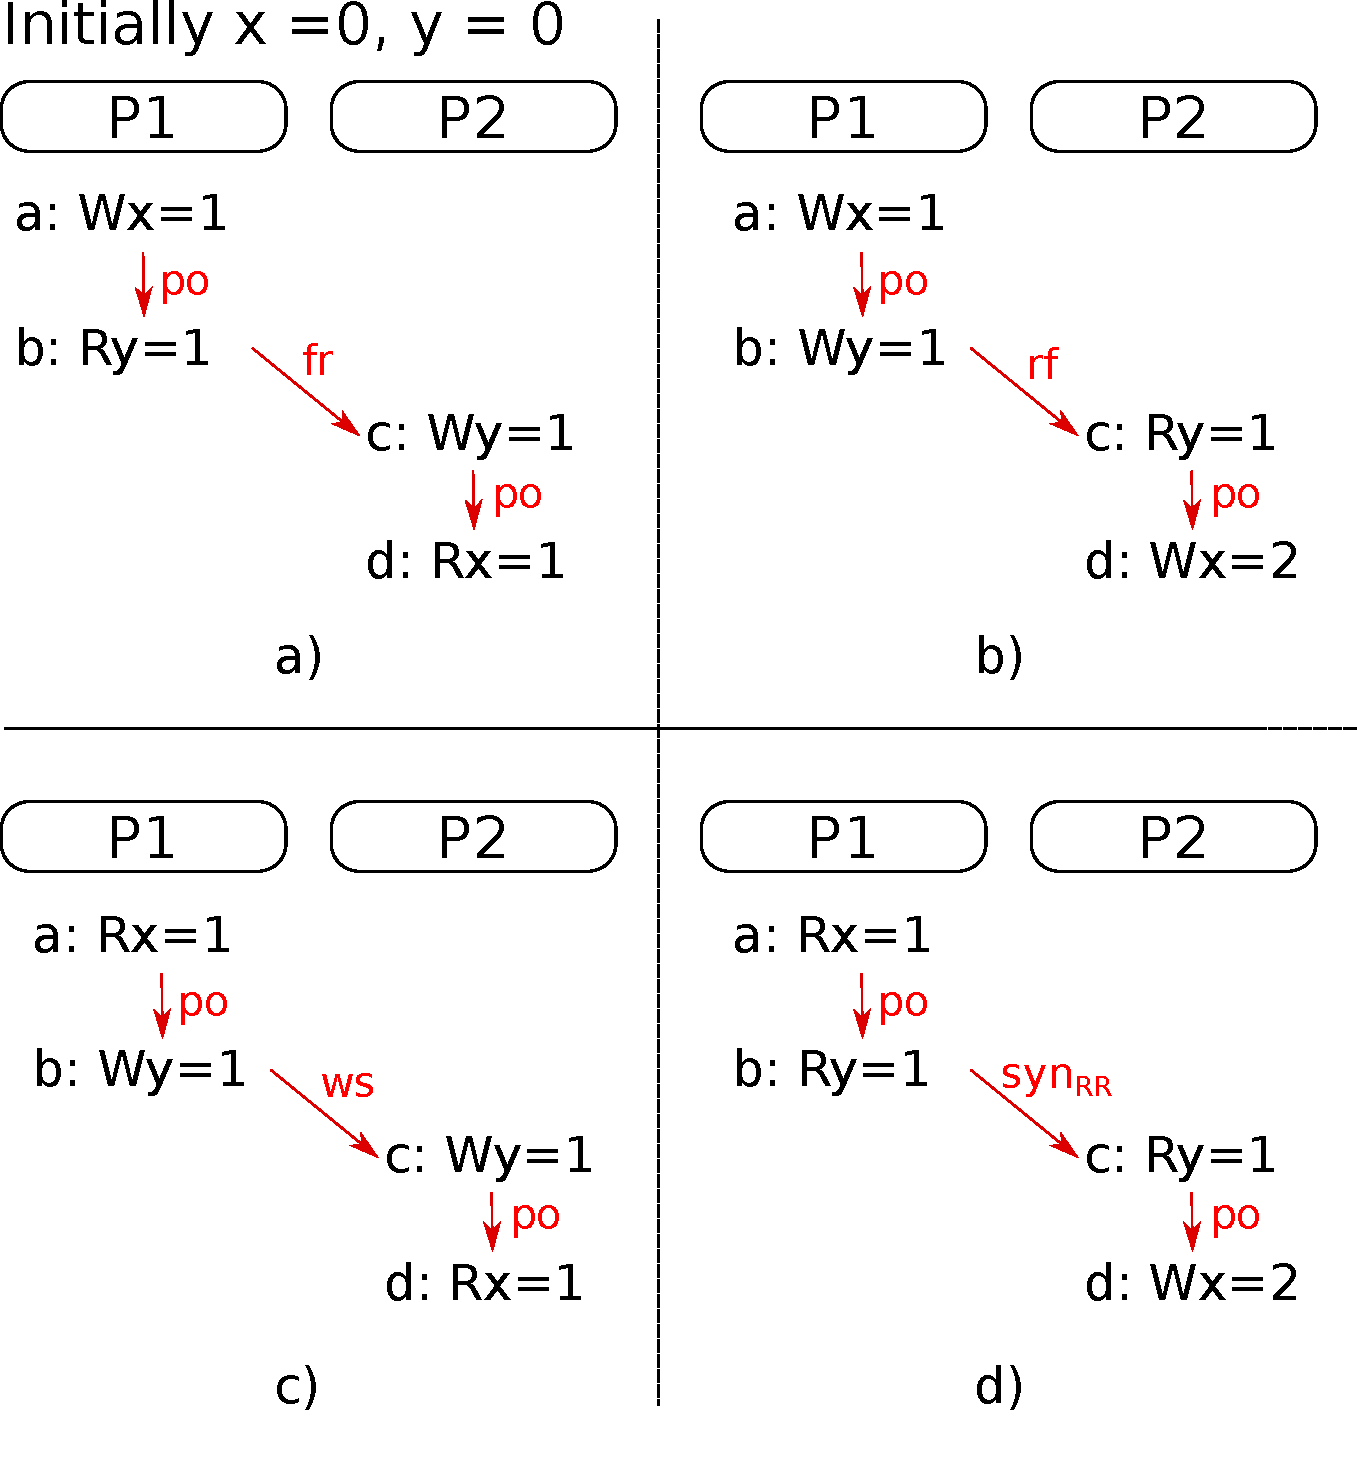
\includegraphics[width=0.28\textwidth]{1_figures/synpat-examples.pdf} 
  \caption{Four examples of \synpats}
  \label{fig:synpat}
\end{figure}


A \synpat\ is a path between two operations to the same object. The path can be constructed through any composition of $\potype$ and $\syntype$ relations, with the only restriction being that at least one $\potype$ must be included (explained in the remarks below).
\tabref{tab:posyn} describes which relations are denoted $\potype$ and $\syntype$.

For example, consider the \synpat\ $s$ that consists of a $\powr$ relation, then an $fr$ relation and then a $\powr$ (depicted in \figref{fig:synpat}a).
We can describe $s$ by composing the three relations as follows:
\begin{equation*}
    s \triangleq \powr ; fr ; \powr
\end{equation*}

Given an execution $E (M, po, rf, hb, RL)$, we assert that $E$ \emph{enforces} $s$ if there exists $rl \in RL$ from which we can derive a $syn$ such that:
\begin{equation*}
    acyclic(s \cup syn)
\end{equation*}
In other words, a \synpat\ that starts from operation $a$ and ends on operation $b$ is said to be \emph{enforced} if $(b, a) \notin syn$.  


\figref{fig:synpat} depicts four \synpats\ to serve as examples.
In the execution of \figref{fig:synpat}a, the $s$ \synpat\ occurs between 
operations $a$ and  $d$. In this instance, $s$ is enforced because $d$ returns the value created by $a$.
If $d$ were to return $0$, that would mean that there is a $syn$ relation between $d$ and $a$ and thus $s$ is not enforced.

\beginbsec{Remarks}
Note the following two remarks. 
First, we use $syn$ rather than $rl$ to test whether a \synpat\ is enforced. This is because the \synpat\ is a path between two operations to the same object, but $rl$ is a total order of all operations across all objects.
Second, note that a \synpat\ must have at least one $\potype$, because otherwise it would just be a composition of $\syntype$ relations. Any such composition is a subset of $syn$, which means that the execution enforces it by definition.

\beginbsec{Consistency models}
An \mcm\ $CM_i$ is defined by asserting that a set
of \synpats\ $S_{CM}$ must be enforced. Plainly, an execution enforces $CM_i$ iff it enforces every $s \in S_{CM}$
As an example, assume that $CM_i$ is defined through the four \synpats\  depicted in \figref{fig:synpat}, which are formalized as follows:
\begin{gather*}
    s_1 \triangleq \powr ; fr ; \powr, \
    s_2 \triangleq \poww ; rf ; \porw, \\
    s_3 \triangleq \porw ; ws ; \powr, \
    s_4 \triangleq \porr ; \synrr ; \porw
\end{gather*}

We define $CM_i$ to be the following rule:
\begin{gather*}
    acyclic(s_1 \cup syn)\
    \andm\ acyclic(s_2 \cup syn)\\ 
    \andm\ acyclic(s_3 \cup syn)\ 
    \andm\ acyclic(s_4 \cup syn)
\end{gather*}






\section{From \mcms\ to \rts}\label{sec:rt-cons}

In this section, we provide a mapping from \mcms\ to \rts.
Specifically,
given an \mcm\ $CM_i$ that is specified through a set $S_{CM}$ of \synpats, we automatically infer a set of \rts, sufficient to enforce $CM_i$. 
In the rest of this section, we first differentiate between regular and irregular \synpats\ (\S\ref{sec:rt-cons:reg}). Then we provide the mapping (\S\ref{sec:rt-cons:map}), prove its correctness for an example \synpat\ (\S\ref{sec:rt-cons:pr}), extend the proof to all regular \synpats\ (\S\ref{sec:rt-cons:reg-ex}) and finally extend the proof to irregular \synpats\ (\S\ref{sec:rt-cons:irreg}).
In \tabref{tab:rt-sGLT}, we provide the mapping of 16 \synpats\ to \rts.
 
\subsection{Regular and irregular \synpats} \label{sec:rt-cons:reg}

We first categorize \synpats\ into two classes: \emph{regular} and \emph{irregular}.
A regular \synpat\ is 1) composed by alternating $\potype$ and $\syntype$ relations and 2) starts and ends on a $\potype$. Thus, any regular \synpat\ $s$, is of the following form:
\begin{equation*}
    s \triangleq \potype ; \syntype; \potype; ...\ \syntype; \potype
\end{equation*}
Any \synpat\ that does not conform to regularity rules is \emph{irregular}.
The distinction between regular and irregular \synpats\ will aid in the  presentation of the mapping from \synpats\ to \rts. Specifically, we will first create a mapping from a regular \synpat\ to the sufficient \rts\ to enforce it. Then, in order to use the same mapping for irregular \synpats, we will show that for every irregular \synpat\ $s_i$, there exists a regular \synpat\ $s_r$, such that enforcing $s_r$ is sufficient to enforce $s_i$. 


\subsection{The mapping} \label{sec:rt-cons:map}

We assert the following three conditions to enforce any regular \synpat, assuming that an operation can be of type $m$ or $n$ where $m, n \in$ $\{read, write\}$.
\squishlist
\item \emph{Cond-1}: for every $\potype$ relation $po_{mn}$ found in $s$, the corresponding \prt\ $prt_{mn}$ must be enforced. Plainly any $\potype$ relation must also be an $hb$ relation. 

\item \emph{Cond-2}: for every $\syntype$ relation $syn_{mn}$, if it is not an $rf$, then the \emph{reverse} \srt\ $srt_{nm}$ must be enforced. 

\item \emph{Cond-3}: if the first operation in $s$ is of type $m$ and the last of type $n$, the corresponding \srt\ $srt_{mn}$ must be enforced.

\squishend

\subsection{Proof for an example \synpat} \label{sec:rt-cons:pr}
We will start by first proving that the three conditions are sufficient for the simple \synpat, that is portrayed in \figref{fig:synpat}a. Then we will extend to any regular \synpat.
The simple \synpat\ $s$ is the following:
\begin{equation*}
    s \triangleq \powr ; fr ; \powr
\end{equation*}
For $s$ the three conditions require the following \rts:
\squishlist
\item \emph{Cond-1}: The $\prtwr$ is required for both $\powr$ relations.

\item \emph{Cond-2}: The $\rtwr$ for the $fr$ (\ie $\synrw$) relation.

\item \emph{Cond-3}: The $\rtwr$ because  $s$ starts with a write and ends on a read.
\squishend

\custvspace
We will show that for any execution \Exec, if $\prtwr$ is enforced and there exists $rl \in RL$ such that $\rtwr$ is enforced then for the $syn$ that is derived from that $rl$ it holds that $acyclic(s \cup syn)$.

To prove this, we first establish a new relation named \emph{begins-before-completes} ($bbc$). 
For two operations $a, b$ we assert that if $b$ does not complete before $a$ begins (\ie $(b, a) \notin hb$), then $a$ begins before $b$ completes (\ie $(a, b) \in bbc$).
We establish the following rule:
\begin{equation*}
 \forall a,d \in M\ s.t.\  (a, d) \in  (hb;bbc;hb) \rightarrow (a,d) \in hb
\end{equation*}
We sketch a proof for this rule using \figref{fig:bbc}a .
\figref{fig:bbc}a illustrates this through
four operations ($a,b,c,d$), each of which is associated with a timestamp ($ta$, $tb$, $tc$, $td$).
Operation $b$ begins before $c$ completes (\ie $(b,c)\in bbc$), while also $(a,b)$, $(c, d)$ $\in hb$. Therefore, $(a, d) \in (hb;bbc;hb)$.
Since $a$ completes before $b$ begins ($ta < tb$) and $b$ begins before $c$ completes ($tb < tc$), it follows that $a$ completes before $c$ completes ($ta < tc$). Because $c$ completes before $d$ begins ($tc < td$), it follows that $a$ completes before $d$ begins ($ta < td$). Therefore, $(a, d) \in hb$.

\figref{fig:bbc}b illustrates the counter-example, where $c$ completes before $b$ begins; in this case it is possible for $d$ to begin before $a$ completes.


\begin{figure}[t]
  \centering
  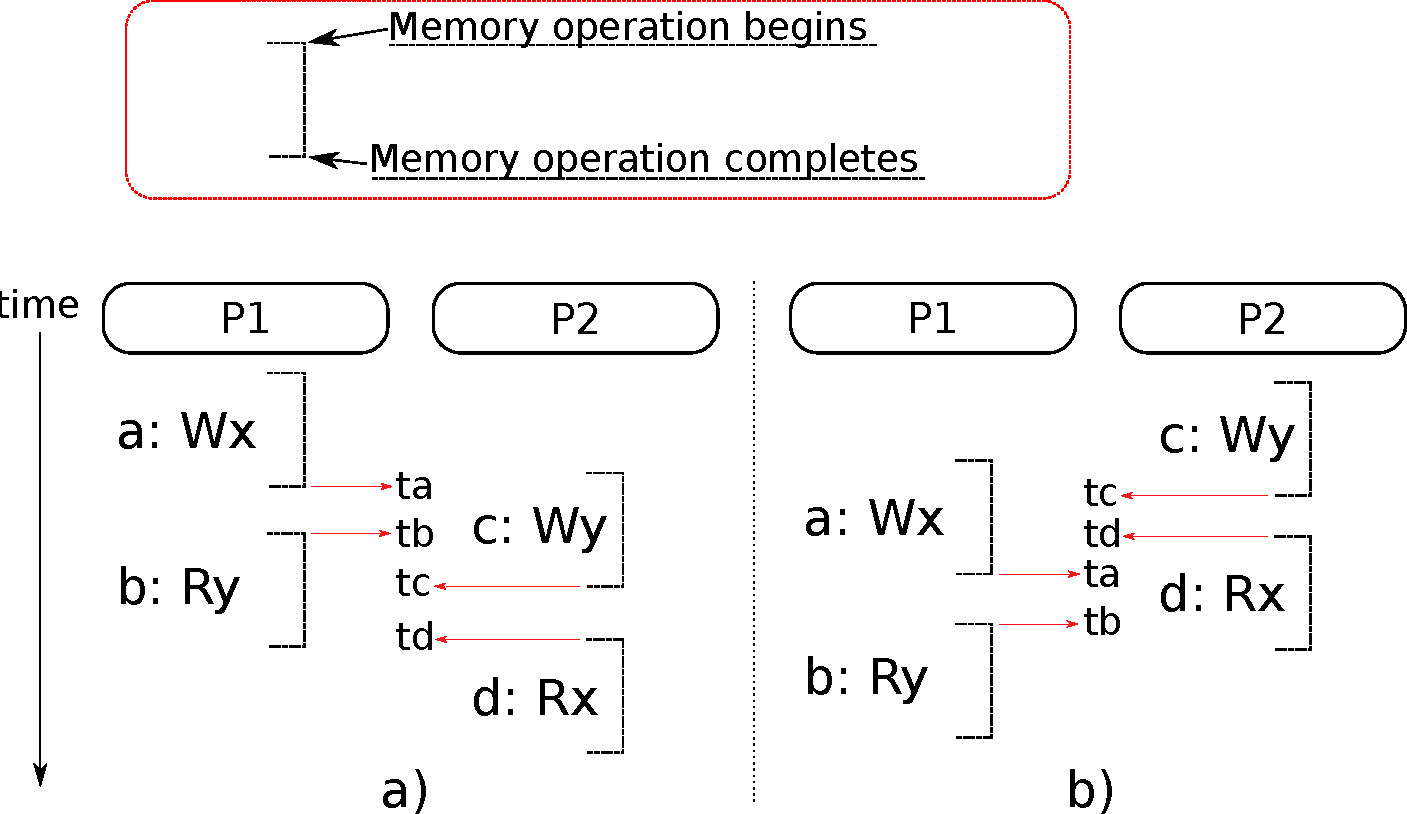
\includegraphics[width=0.35\textwidth]{1_figures/hb-bbc-hb.pdf}
  \caption{a) $b$ begins before $c$ completes  b) $c$ completes before $b$ begins. }
  \vspace{-1em}
  \label{fig:bbc}
\end{figure}


Consider an execution \Exec, for which there exists an $rl \in RL$ such that all three conditions we asserted are satisfied.
Assume four operations $a,b,c,d \in M$ such that $(a, b) \in \powr \andm (b,c) \in \synwr \andm (c,d) \in \powr$. This implies that $(a, d) \in s$.
Let us now assume that 
$(a, d) \in  (hb;bbc;hb)$ and thus $(a,d) \in hb$. Specifically, $(a,d) \in \hbwr$. This is illustrated in \figref{fig:bbc}a.
From the cond-3 ($\rtwr$), we can assert that since $(a,d) \in \hbwr$ it follows that $(d, a) \notin syn$ and thus it must be that $acyclic(s \cup syn)$.
Plainly, cond-3 ensures that  $acyclic(s \cup syn)$ if  the following condition holds: 
\begin{equation*}
 \forall a,d \in M\ s.t.\  (a, d) \in  s \rightarrow (a,d) \in hb
\end{equation*}
Therefore it suffices to prove that cond-1 and cond-2 guarantee the above condition. We will do so by proving that $(a, d) \in (hb;bbc;hb)$.

Firstly, cond-1 ($\prtwr$) mandates that $\powr \subseteq \hbwr$.
Therefore, $(a, b)$, $(c, d) \in hb$. 
We need only prove that $(b, c) \in bbc$. 
Let's assume that $(b, c) \notin bbc$. It follows that $(c, b) \in hb$.
Recall, that $b$ is a write and $c$ is a read. Cond-2 mandates that $\rtwr$ is enforced: since $(c, b) \in hb$ then $(b, c) \notin syn$. 
We have reached a contradiction, and therefore it must be that $(b, c) \in bbc$.

\figref{fig:bbc}b provides the counter example where $(b, c) \notin bbc$.
In this case it cannot be that $(a,d) \in s$ because $(b, c) \in hb$ and therefore from cond-2 it follows that $(c, b) \in syn$. Plainly, the \synpat\ $s$ will not occur here because P1's read to $y$ will observe P2's write to $y$.

As we have shown above, from cond-1 and cond-2 it follows that $(a, d) \in  hb$ and thus from cond-3 it follows that $(a, d) \notin syn$. Therefore the three conditions are sufficient to enforce $s$.

\subsection{Extending to all regular \synpats} \label{sec:rt-cons:reg-ex}
Note the intuition behind the three conditions. Cond-1 ensures that every $\potype$ relation of the \synpat\ is also an $hb$ relation. Similarly, cond-2 ensures that every $\syntype$ relation is also a $bbc$ relation. As a regular \synpat\ is composed by alternating $\potype$ and $\syntype$ relations, enforcing cond-1 and cond-2 ensures that the \synpat\ can be expressed as a composition of alternating $hb$ and $bbc$ relations.

As we saw $hb;bbc;hb \subseteq hb$. By induction we can extend this rule for any sequence of alternating $hb$ and $bbc$ relations. Specifically:
\begin{equation*}
\forall a,b \in M\ s.t.\ (a, b) \in hb;bbc;hb\ ....\ hb;bbc;hb \rightarrow (a,b) \in hb
\end{equation*}
Therefore, cond-1 and cond-2 ensure that if $(a, b) \in s$ then $(a,b) \in hb$ for any regular \synpat\ $s$. Finally, cond-3 ensures that the \synpat\ is enforced, by ensuring that if $(a,b) \in hb$ then $(b,a) \notin syn$.
This means that our three conditions can be used to enforce any regular \synpat.

\beginbsec{Examples -- \tabref{tab:rt-sGLT}}
\tabref{tab:rt-sGLT} depicts the sufficient \rts\ for 16 \synpats. Specifically, each cell represents a distinct \synpat\ between operations $a,b,c,d$. For instance, the highlighted cell where $a = Wx$, $b = Ry$, $c = Wy$, $d = Rx$, corresponds to the \synpat\ of \figref{fig:synpat}a.

\beginbsec{Cond-2 exception: $\mathbf{rf}$}
Recall that cond-2 is not required for $rf$ edges. This is because the purpose of cond-2 is to ensure that the $\syntype$ relation is also a $bbc$ relation. However, this is implied by the $rf$ as it is impossible for a read $r$ to read-from a write $w$ if $r$ completes before $w$ begins. Plainly: 
$\forall w,r \in M\ s.t.\  (w,r) \in rf \rightarrow (w,r) \in bbc $.
    
\beginbsec{Producer-consumer (\figref{fig:intro-ex}a)}
Let $s_{pc}$ be the producer-consumer \synpat\ of \figref{fig:intro-ex}a (discussed in the Introduction). We assert that $s_{pc} \triangleq \poww; rf;\porr$. To enforce $s_{pc}$, cond-1 requires \prts\ $\prtww, \prtrr$, cond-2 does not require any \srt\ because the only $\syntype$ is an $rf$ and cond-3 requires the $\rtwr$.




\begin{table}[t]
\centering
\footnotesize
 \resizebox{0.48\textwidth}{!}{%
\begin{tabular}{c|c|c|c|c|}
\hhline{~----}
                                                        
 & 
\headercell{c = Wy \\ d = Ry} &
\headercell{c = Wy\\ d = Wy} &
\headercell{c = Ry\\ d = Ry} &
\headercell{c = Ry\\ d = Wy}
\\ \hline
\multicolumn{1}{|c|}{
\headercell{a = Wx\\ b = Rx}} & 
\cellcolor[HTML]{9AFF99}  \itcell{$\rtwr$, \\ $\prtwr$}&
\itcell{$\rtww$, $\rtwr$, \\ $\prtwr$, $\prtww$}  &
\itcell{$\rtwr$,  $\rtrr$, \\ $\prtwr$, $\prtrr$}  & 
\itcell{$\rtww$,  $\rtrr$, \\ $\prtwr$, $\prtrw$}                                                         
\\ \hline
\multicolumn{1}{|c|}{
\headercell{a = Wx\\ b = Wx}} & 

\itcell{$\rtwr$, $\rtww$, \\$\prtww$, $\prtwr$}&
\itcell{$\rtww$, \\$\prtww$}  &
\itcell{$\rtwr$,  $\rtrw$, \\$\prtww$, $\prtrr$}  & 
\itcell{$\rtww$,  $\rtrw$, \\$\prtww$, $\prtrw$}  
\\ \hline
\multicolumn{1}{|c|}{
\headercell{a = Rx\\ b = Rx}} &

\itcell{$\rtrr$, $\rtwr$, \\ $\prtrr$, $\prtwr$}&
\itcell{$\rtrw$, , $\rtwr$, \\ $\prtrr$, $\prtww$}  &
\itcell{$\rtrr$, \\ $\prtrr$}  & 
\itcell{$\rtrw$,  $\rtrr$, \\ $\prtrr$, $\prtrw$}  
\\ \hline
\multicolumn{1}{|c|}{
\headercell{a = Rx\\ b = Wx}} &
\itcell{$\rtrr$, $\rtww$, \\ $\prtrw$, $\prtwr$}&
\itcell{$\rtrw$, , $\rtww$, \\ $\prtrw$, $\prtww$}  &
\itcell{$\rtrr$ ,  $\rtrw$, \\ $\prtrw$, $\prtrr$}  & 
\itcell{$\rtrw$, \\ $\prtrw$}  
\\ \hline
\end{tabular}%
}
\caption{The mapping of 16 \synpats\ to \rts. Each cell represents a \synpat\ of the form $s \triangleq \potype ; \syntype; \potype$, where the first $\potype$ includes $(a,b)$, the $\syntype$ includes $(b,c)$ and the second $\potype$ includes $(c,d)$. The highlighted cell corresponds to \figref{fig:synpat}a.}%
 \vspace{-1em}
\label{tab:rt-sGLT}
\end{table}

\subsection{Extending to irregular \synpats}\label{sec:rt-cons:irreg}

A \synpat\ is deemed \emph{irregular} if 1) it has consecutive $\potype$ relations or 2) it has consecutive $\syntype$ relations or 3) it does not start with a $\potype$ relation (\ie starts with $\syntype$) or 4) it does not end with a $\potype$ relation (\ie ends with $\syntype$).
For each such \synpat\ $s$, we derive a \synpat\ $s'$ such that 1) $s'$ is regular and 2) if $s'$ is enforced then $s$ must also be enforced.



\beginbsec{Consecutive po-type}
We start with \synpats\ with consecutive $\potype$ relations.
We use the insight that any composition of $\potype$ relations must be the subset of one of $\poww$, $\powr$, $\porr$, $\porw$ relation. 
For instance $\poww;\powr;\porr;\porw$ is a subset of $\poww$. Therefore, for any $s$ that has consecutive composed $\potype$ relations, we derive a $s'$ which replaces them with a single $\potype$ relation, such that $s \subseteq s'$ and we assert that enforcing $s'$ is sufficient to also enforce $s$. Below is an example of $s$ and the derived $s'$ using the insight that 
$(\powr ; \porw) \subseteq \poww$.
\begin{gather*}
    s \triangleq \powr ; \porw; \synwr; \porr \\
    s' \triangleq \poww; \synwr; \porr
\end{gather*}



Note that an alternative approach would have been to omit deriving $s'$ and instead simply asserting that the first condition is applied for each $\potype$ relation in $s$. That would still be correct and can be used.

\beginbsec{Consecutive syn-type}
Our approach is identical for \synpats\ with consecutive composed $\syntype$ relations. Specifically, a composition of $\syntype$ relations is always a subset of one of $fr$, $ws$, $\synwr$, $\synrw$. This is because 
any pair in a composition of $\syntype$ relations is also in $syn$ and thus it must be in one of $fr, ws, \synwr \synrw$, as $syn$ is the union of these four relations.
Therefore, for any $s$ that has consecutive composed $\syntype$ relations, we derive an $s'$ which replaces them with a single $\syntype$ relation, such that $s \subseteq s'$.

\beginbsec{Begin with syn-type}
When a \synpat\ $s$ begins with a $\syntype$ relation, then we derive $s'$ by simply removing it.
Let us see why through an example.
Assume the following $s$ which starts with an $fr$ and the derived $s'$ which removes the $fr$:
\begin{gather*}
    s\triangleq fr ; \powr fr; \powr \\
    s' \triangleq\powr fr; \powr
\end{gather*}
Assume now that $(a,c) \in s$,  $(b,c) \in s'$ and $(a, b) \in fr$.
Let us now prove that if $s'$ is enforced, $s$ is enforced too.
Assume $s'$ is enforced but $s$ is not. Therefore, $(c,b) \notin syn$ but $(c, a) \in syn$. We know that $(a, b) \in fr$ and thus $(a, b) \in syn$. By the transitivity property of $syn$ we assert that since $(c, a) \in syn \andm (a, b) \in syn$ it must be that $(c, b) \in syn$. This contradicts our assumption that $s'$ is enforced.
Therefore enforcing $s'$ is sufficient to also enforce $s$.

\beginbsec{End on syn-type}
Similarly, if $s$ ends on a $\syntype$ relation, we remove it to derive $s'$.
Assume the following example.
\begin{gather*}
    s\triangleq \powr fr; \powr fr\\
    s' \triangleq\powr fr; \powr
\end{gather*}
Assume now that $(a,c) \in s$,  $(a,b) \in s'$ and $(b, c) \in fr$.
Using the same proof as above, we can infer that if $s'$ is enforced then $(b,a) \notin syn$ and thus it follows that $(c, a) \notin syn$. Therefore enforcing $s'$ is sufficient to also enforce $s$.

\beginbsec{A combination of the above (IRIW -- \figref{fig:intro-ex}b)}
When a \synpat\ falls into more than one of the above irregular categories, we combine the techniques discussed above. For instance, let $s_{iriw}$ be the IRIW \synpat\ of \figref{fig:intro-ex}b (discussed in the Introduction). 
\begin{equation*}
    s_{iriw} \triangleq rf;\porr;fr;rf;\porr
\end{equation*}
This is an irregular \synpat, which both starts with a $\syntype$ and includes a composition of consecutive $\syntype$ relations. We use the rules above to derive $s_{iriw}'\triangleq \porr;\synrr\porr$ and assert that if $s_{iriw}'$ is enforced then $s_{iriw}$ is also enforced.
To enforce $s_{iriw}'$, cond-1 requires the \prt\ $\prtrr$ and cond-2 requires the \srt\ $\rtrr$ which is also required by cond-3.












\section{From \rts\ to \mcms} \label{sec:rt-to-cons}
So far we have created a mapping from \mcms\ to \rts, by establishing the sufficient \rts\ to enforce any \synpat.
In this section, we use this result to obtain the reverse mapping from \rts\ to \mcms,  focusing our discussion solely on regular \synpats, seeing as the enforcement of irregular \synpats\ is done by mapping them to regular ones.
To obtain the mapping from \rts\ to \synpats, we reverse each of the three conditions, assuming that an operation can be of type $m$ or $n$ where $m, n \in$ $\{read, write\}$. Specifically, given a protocol that enforces a set of \prts\ $R_p$ and a set of \srts\ $R_s$, a \synpat\ $s$ is enforced when it abides by the following conditions:


\squishlist
\item \emph{Cond-1$'$} : $s$ can include a $\potype$ relation $po_{mn}$ if $prt_{mn} \in R_p$.
\item \emph{Cond-2$'$}: $s$ can include a $\syntype$ relation $syn_{mn}$ if it is an $rf$ relation or $srt_{nm} \in R_s$. 
\item {Cond-3$'$}: $s$ can start with an operation of type $m$ and end on an operation of type $n$, if $srt_{mn} \in R_s$.
\squishend

\beginbsec{Example}
To showcase how these conditions can be used in practice, let us specify the \mcm\ $CM_{i}$ that is enforced by a protocol that enforces the rt-orderings $\prtww, \prtwr, \rtrw$ and $\rtwr$.  %
To do so we must specify a set of \synpats\ $S_{CM}$  where each regular \synpat\ $s \in S_{CM}$ abides by the following rules:
\squishlist
\item Any $\potype$ relation in $s$ is either a $\poww$ or a $\powr$
\item Any $\syntype$ relation in $s$ is either a $\synwr$ or a $\synrw$. ($rf$ is included in $\synwr$)
\item $s$ must either start on a write and end on a read, or start on a read and end on a write.
\squishend

Notably, the interplay amongst the rules can be used to further simplify them. For instance the third rule asserts that from the available \srts\ ($\rtrw$ and $\rtwr$) it follows that either the first operation must be a read and the last a write or the reverse. However, neither of the available $\potypes$ ($\poww$ and $\powr$) start with a read and since a regular \synpat\ must start with a $\potype$ relation, it cannot be that the first operation is a read. Consequently, the first operation can only be a write, and thus the last operation must be a read, to abide by the third rule. 


Similarly, because a regular \synpat, is a composition of alternating $\potype$ and $\syntype$ relations, it follows that the available $\potype$ and $\syntype$ relations can only be used if they can synergize. For instance, the $\synwr$ cannot be used at all because neither of the available $\potypes$ ($\poww$ and $\powr$) starts from a read.
Similarly, because the $\synwr$ cannot be used, the $\poww$ cannot be used before any $\syntype$, nor can it be used as the last relation because the \synpat\ must end on a read. 

\custvspace
\noindent Therefore the rules for a \synpat\ $s \in S_{CM}$ are simplified as follows:
\squishlist
\item Any $\potype$ relation in $s$ must be a $\powr$
\item Any $\syntype$ relation in $s$ must be a $\synrw$. 
\item $s$ must start on a write and end on a read.
\squishend


As a result any regular  \synpat\ $s \in S_{CM}$ is a composition of alternating $\powr$ ans $\synrw$ relations. Below, we list a few examples \synpats\ in $S_{CM}$
\begin{gather*}
    s_{1} \triangleq \powr ; \synrw; \powr \\
    s_{2} \triangleq \powr ; \synrw; \powr; \synrw; \powr\\
    s_{3} \triangleq \powr ; \synrw; \powr;\ ...\ \synrw; \powr
\end{gather*}


Notably, enforcing the $\prtww$ and $\rtrw$ are not contributing towards enforcing any $s \in S_{CM}$. 



\section{From \rts\ to Protocols} \label{sec:prot}

In previous sections we established the mappings between the \synpats\ and the \rts. 
In this section, we relate \rts\ to some well-known protocol design techniques. %
We start with a brief discussion on the \prts\ and then we focus on the \srts.






\subsection{Enforcing \rts}
\Prts\ model the operation of the \rob\ specifying  when the memory system can begin executing an operation.
Upholding the \prts\ is as simple as inspecting the state of the \rob.
For instance, enforcing $\prtwr$ implies that the memory system cannot begin executing a read $r$ from process $p$, until every preceding write in the \rob\ is completed.



\custvspace
\Srts\ models how the memory system executes reads and writes.
Below we discuss two common techniques that can be used to enforce \srts\ 1) \emph{overlap} and 2) \emph{lockstep}.

\beginbsec{Overlap}
The \srt\ $srt_{mn}$ can be enforced simply by ensuring that operations of type $m$ must overlap with operations of type $n$ in a physical location. For instance, we can enforce $\rtwr$, by ensuring that a write is propagated to $x$ nodes and a read queries $y$ nodes, where $x+y > N$ and $N$ is the number of nodes. 
Alternatively, both types of operations can \qt{meet} in some centralized physical location (\eg the directory for multiprocessors). 
To ensure all four \srts\ and thus linearizability, both reads and writes must query $y$ nodes to learn about completed operations and must broadcast their results to $x$ nodes. This is exactly how the multi-writer variant of ABD~\cite{Lynch:1997} operates.

\beginbsec{Lockstep}
Lockstep is %
a technique, %
where a memory system node first \qt{grabs a lock} on the object before beginning an operation and releases it when the operation completes. 
Upon grabbing the lock, the node learns about the operation executed by the previous lock holder.
The act of \qt{grabbing the lock} is similar to getting a cache-line in $M$ or $S$ state in a coherence protocol~\cite{Vijay:2020}, or becoming the leader of the next log entry in a state machine replication protocol, such as Paxos~\cite{Lamport:1998}. Notably, lockstep entails overlap as operations must meet in a physical location to exchange the lock, but it also precludes the operations from executing concurrently.

There are two aspects of lockstep that can enforce \srts.
First, the \srt\ between two operations is enforced if a lock must be passed from one to the other. 
For example we can enforce $\rtww$ by mandating that a lock must be grabbed to perform a write.
Second, locking also ensures that certain operations cannot overlap in real-time.
When a write cannot overlap with a write and $\rtww$ is enforced then $\rtrw$ is also enforced. This is because if a read $r$ returns the value of write $w$, then a write $k$ that begins after $r$ has completed must also begin after $w$ has completed.
Similarly, when a write cannot overlap with a read and $\rtwr$ is enforced, then $\rtrr$ is enforced. This is because if a read $r$ returns the value of write $w$, then it must be that $w$ completes before $r$ begins. Therefore, a read $m$ that begins after $r$ has completed, must also begin after $w$ has completed and thus will observe $w$.
Protocols often combine the two aspects of lock-step to enforce the single-writer multiple-reader invariant (\SWMR)~\cite{Vijay:2020}, where for any given object at any given time there is either a single write in progress or multiple reads.
This ensures that writes must grab a lock from each other ($\rtww$), reads must grab a lock from writes ($\rtrw$), writes cannot overlap in time ($\rtrw$) and writes do not overlap in time with reads ($\rtrr$).





\section{Discussion} \label{sec:disc}
In this work, we have used the \rts\ to model the protocol, allowing us to create a mapping from MCMs to protocols. In this section, we discuss other use-cases of the \rts. We start by describing the relation of \srts\ to linearizability and then we discuss  how they can be used to describe the real-time guarantees of existing protocols and to decide the consistency guarantees provided when protocols are composed.

\subsection{Relation of \srts\ to linearizability}\label{disc:lin}
Formally, the lin criterion~\cite{Herlihy:1990} can be written in our notation as follows.
An execution \Exec\ is linearizable if there exists $rl \in RL$ such that $hb \subseteq rl$. Furthermore, because lin is a \emph{local} property, it suffices that only operations to the same object abide by the rule. Plainly, for two operations $a,b$ to the same object $x$, if $(a,b) \in hb$ then it must be that $(a,b) \in rl$. This is equivalent to: $acyclic(hb, syn)$.
This, in turn, is equivalent to enforcing all four \srts.
Therefore, the lin property is the property of enforcing all four \srts.


\beginbsec{Intuition}
Informally, the lin property can be defined by writing that \emph{each memory operation appears to take effect at some point between its invocation and completion}~\cite{Herlihy:2008}.
Notably, each of the \srts\ is a specialization of this definition.
For instance, $\rtwr$ mandates that each write appears to take effect at some point between its invocation and completion w.r.t. every read.
Combining all four \srts\ mandates that each write or read appears to take effect at some point between its invocation and completion w.r.t. every read or write. This is equivalent to the lin definition.

\subsection{\Srts\ for compositionality}\label{disc:cons}

So far we have viewed the \srts\ solely as a mathematical model of the protocol.
However, in distributed systems, it is often necessary to describe the real-time guarantees offered by a system, in order to compose different systems.
Consider the example of Zookeeper. Zookeeper does not offer linearizability, and thus multiple Zookeeper instances cannot be composed. However, researchers have found that Zookeeper does offer some real-time guarantees that can be leveraged to achieve compositionality~\cite{LevAri:2016}.

\Srts\ can be used to capture these real-time guarantees. For example, the precise real-time guarantees of Zookeeper are the $\rtww$ and the $\rtrw$ \srts and all four \prts.
More importantly, given this knowledge we can specify the MCM provided by composing different Zookeeper instances: the composed system will enforce the same \rts\ as a single Zookeeper instance and thus we can use the reverse mapping from \rts\ to \synpats\ to specify the resulting MCM. In fact, we can use \srts\ in the same spirit, to specify the MCM of any combination of composed systems, by asserting that the composed system will enforce any \rt\ that is enforced by all of its subsystems.







\section{Related Work} \label{sec:related}



This work is the first to provide a mapping from \mcms\ to the protocols that can enforce them. To present this mapping we have used an abstract system model and the formalism presented by Alglave \etal~\cite{Alglave:2014} in order to describe \mcms, executions and real-time guarantees. Several works~\cite{Szekeres:2018,Crooks:2017, Burckhardt:2014, LevAri:2017, Gotsman:2017} have also described similar system models and formalism, but differ from our work in that they do not provide a mapping from \mcms\ to the protocols.
Specifically, Szekeres and Zhang~\cite{Szekeres:2018} provide a system model and a formalism called \emph{result visibility} to describe consistency guarantees, including real-time guarantees.
Crooks \etal\cite{Crooks:2017}, focusing on databases, provide a state-based formalization of isolation guarantees.
Burckhardt, in his book on Eventual Consistency~\cite{Burckhardt:2014}, provides a formalism to describe consistency models and protocols, with a focus on weaker guarantees.
Lev-ari \etal~\cite{LevAri:2017} define Ordered Sequential Consistency, OSC(A), in order to specify the real-time guarantees of a protocol (with a focus on Zoo\-kee\-per~\cite{Hunt:2010}). 
Similarly, Gotsman  and  Burckhardt propose GSC~\cite{Gotsman:2017}, a generic operational model for systems that totally order all writes, which can capture all of the \srts\ for such systems.


\custvspace
In the cache coherence literature, the four \emph{program-orderings} are used to describe consistency guarantees~\cite{Vijay:2020}. In fact, 
researchers have shown that when the coherence protocol enforces the \emph{single-writer multiple-reader} (\SWMR) invariant, the \mcm\ depends solely on the enforced program orderings~\cite{Arvind:2006, Meixner:2005}.
Program orderings are very similar to \prts\ with the subtle difference that program orderings carry the implication that the memory system enforces \SWMR. In contrast, \prts\ make no such assumption, allowing us to explore all possible behaviours of the memory system.

Finally, CCICheck~\cite{Manerkar:2015} provides a way to verify an existing coherence protocol against its target \mcm\ using the notion of μhb orderings, which are related to real-time.
Our work provides a mapping from \mcms\ to protocols, enabling the design of minimal protocols for any \mcm.
























\section{Conclusion and Lessons Learned}
\label{sec:conclusion}

The goal of the paper is to uncover the impact of modern hardware on the performance of strongly-consistent replication protocols.
To this end, we presented \odlib, a framework that enables the fast development and deployment of replication protocols over modern hardware. 
Over \odlib, we built and evaluated \pnum\ protocols. 
Extrapolating their results to the entire design space through an informal taxonomy, we provided a characterization of strongly-consistent replication protocols.

On the system side, we experienced first-hand the necessity for a reliable, high-performance framework to design, build and deploy replication protocols. Without it, system-level bugs (networking, KVS etc.) become a black hole for developer time.
In hindsight, this is no surprise: clean interfaces that abstract orthogonal components have been the cornerstone of computer science. %
Nevertheless, 
we were pleasantly surprised to see that we can build and deploy a new protocol in two days (\S\ref{sec:why}). 

When it comes to protocol design, the overarching lesson is that the true limits of a protocol will be uncovered only when all artificially imposed bottlenecks have been removed. 
Plainly, this calls for highly-optimized, multi-threaded and \RDMA-enabled implementations. 
It is very telling that ZAB outperforms Classic Paxos (CP) by more than 2x when both are single-threaded, but the result is inverted when they are multi-threaded. 
The pseudo bottleneck of single-thread implementations conceal ZAB's inefficiencies while holding back CP's capabilities. Multi-threading removes the bottleneck, laying bare the true nature of the protocols.






\begin{acks}
 We would like to thank the anonymous reviewers for their valuable comments and Dan Sorin for the insightful discussions and valuable feedback.
 This work was supported in part by EPSRC grant EP/L01503X/1 to The University of Edinburgh and ARM through its PhD Scholarship Program.
\end{acks}




\bibliographystyle{IEEEtranS}
\bibliography{paper}




\end{document} 
